\documentclass[12pt]{article}
\usepackage[utf8]{inputenc}
\usepackage[T1]{fontenc}
\usepackage[margin=2.5cm]{geometry}
\usepackage{graphicx}
\usepackage{booktabs}
\usepackage{longtable}
\usepackage{multirow}
\usepackage{float}
\usepackage{subcaption}
\usepackage{fancyhdr}
\usepackage{enumitem}
\usepackage{titlesec}
\usepackage{hyperref}
\usepackage[backend=biber,style=apa]{biblatex}
\usepackage{url}
\addbibresource{references.bib}

% Header and footer setup
\pagestyle{fancy}
\fancyhf{}
\rhead{Netflix Viewing Analysis}
\lhead{Buse Özcan}
\rfoot{Page \thepage}

% Section formatting
\titleformat{\section}
{\normalfont\Large\bfseries}{\thesection}{1em}{}
\titlespacing*{\section}{0pt}{3.5ex plus 1ex minus .2ex}{2.3ex plus .2ex}

\title{\textbf{Analysis of Personal Netflix Viewing Habits\\(2020-2024)}\\
\large A Data Science Perspective on Entertainment Consumption Patterns}
\author{Buse Özcan}
\date{\today}

\begin{document}
\maketitle
\thispagestyle{empty}

\begin{abstract}
This comprehensive analysis examines personal Netflix viewing patterns over a four-year period (2020-2024), providing detailed insights into entertainment consumption habits. The study analyzes 1,395 viewing sessions across 162 unique series and movies, investigating temporal patterns, content preferences, and binge-watching behavior. Through statistical analysis and data visualization, this report reveals significant patterns in viewing habits, genre preferences, and binge-watching behavior. Key findings highlight strong preferences for specific genres and series, distinct temporal viewing patterns, and notable binge-watching behaviors that characterize modern streaming consumption habits.
\end{abstract}

\newpage
\tableofcontents
\newpage

\section{Introduction}
\subsection{Study Overview}
This analysis explores personal Netflix viewing habits using detailed viewing history data from 2020 to 2024. The study aims to understand patterns in content consumption, identify viewing preferences, and analyze binge-watching behavior through quantitative analysis of viewing records.

\subsection{Data Collection}
The dataset comprises complete Netflix viewing history records, including:
\begin{itemize}[noitemsep]
    \item Viewing timestamps and durations
    \item Series and episode information
    \item Content metadata (genres, ratings, languages)
    \item Completion status for series
\end{itemize}

\section{Methodology}
The analysis employs various analytical approaches:
\begin{itemize}
    \item Temporal pattern analysis across multiple time scales
    \item Genre preference identification and categorization
    \item Binge-watching behavior detection and analysis
    \item Series completion rate calculations
    \item Content rating analysis
\end{itemize}

\section{Overall Viewing Statistics}
\subsection{Key Metrics}
The analysis revealed several fundamental patterns in viewing behavior:
\begin{itemize}
    \item Total Viewing Sessions: 1,395
    \item Unique Content Items: 162
    \item Average Daily Episodes: 1.00
    \item Weekend Viewing Ratio: 27.38\%
    \item Total Binge Sessions: 291
    \item Average Episodes per Binge: 3.66
\end{itemize}

\subsection{Temporal Distribution}
\begin{figure}[H]
\centering
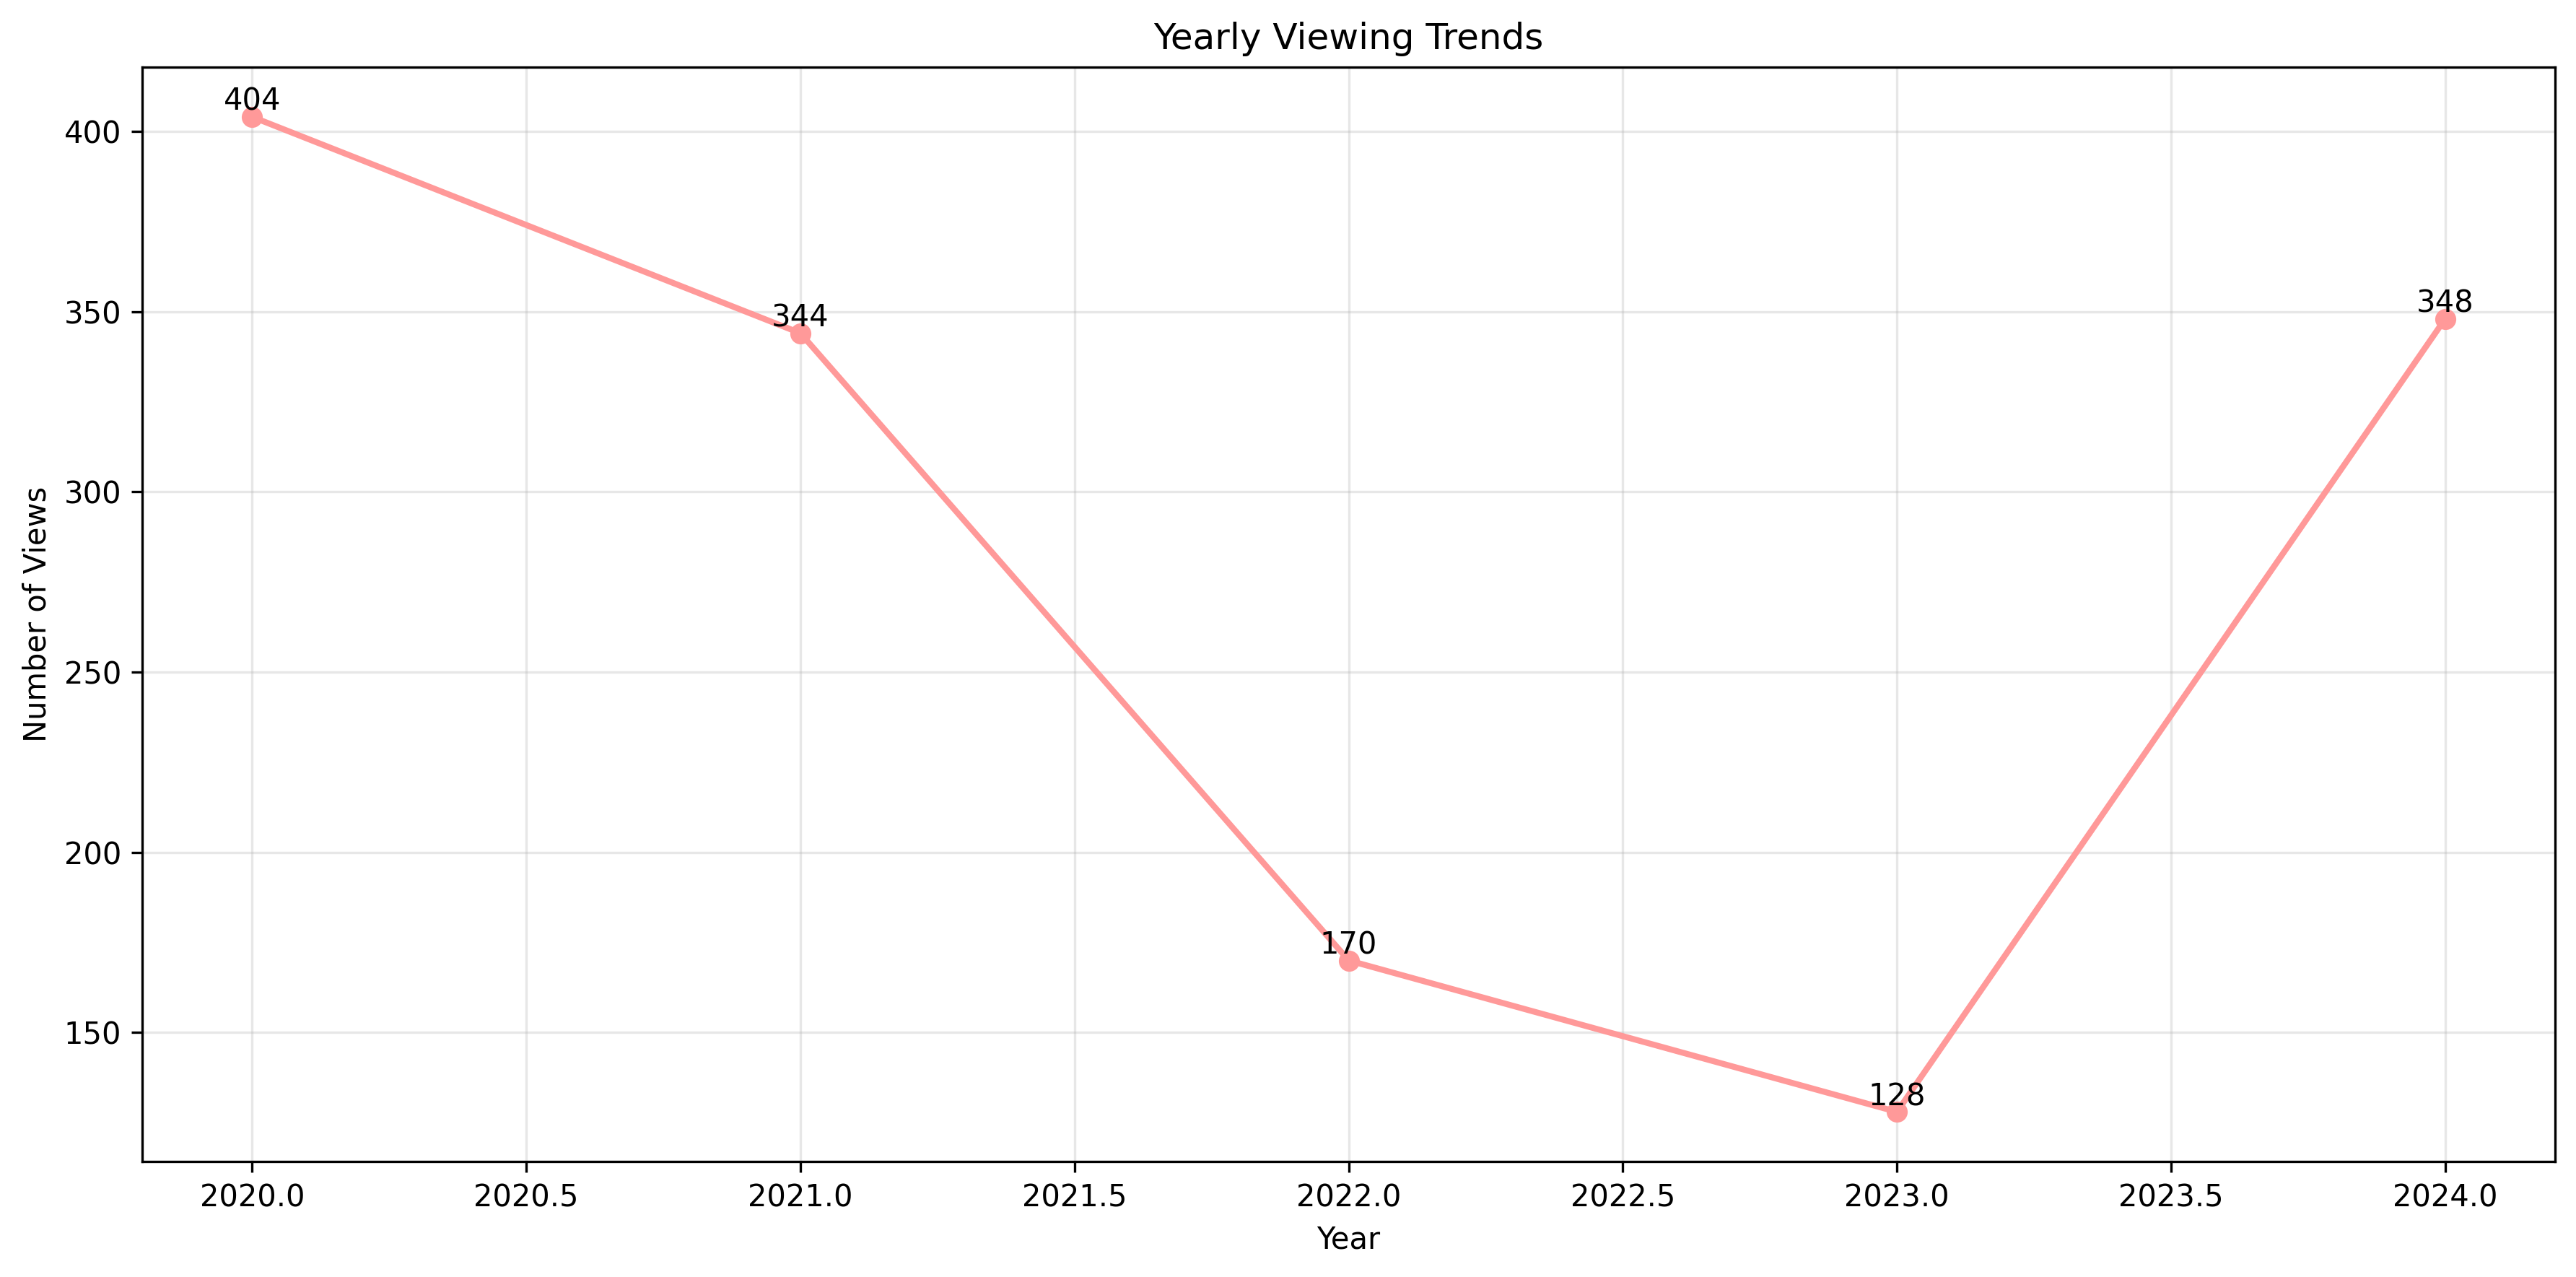
\includegraphics[width=0.8\textwidth]{yearly_trends.png}
\caption{Yearly Viewing Distribution (2020-2024)}
\label{fig:yearly_trends}
\end{figure}

The yearly distribution analysis (Figure \ref{fig:yearly_trends}) shows significant variations in viewing intensity across different years, with 2020 showing the highest activity levels, possibly influenced by global lockdown measures.

\begin{figure}[H]
\centering
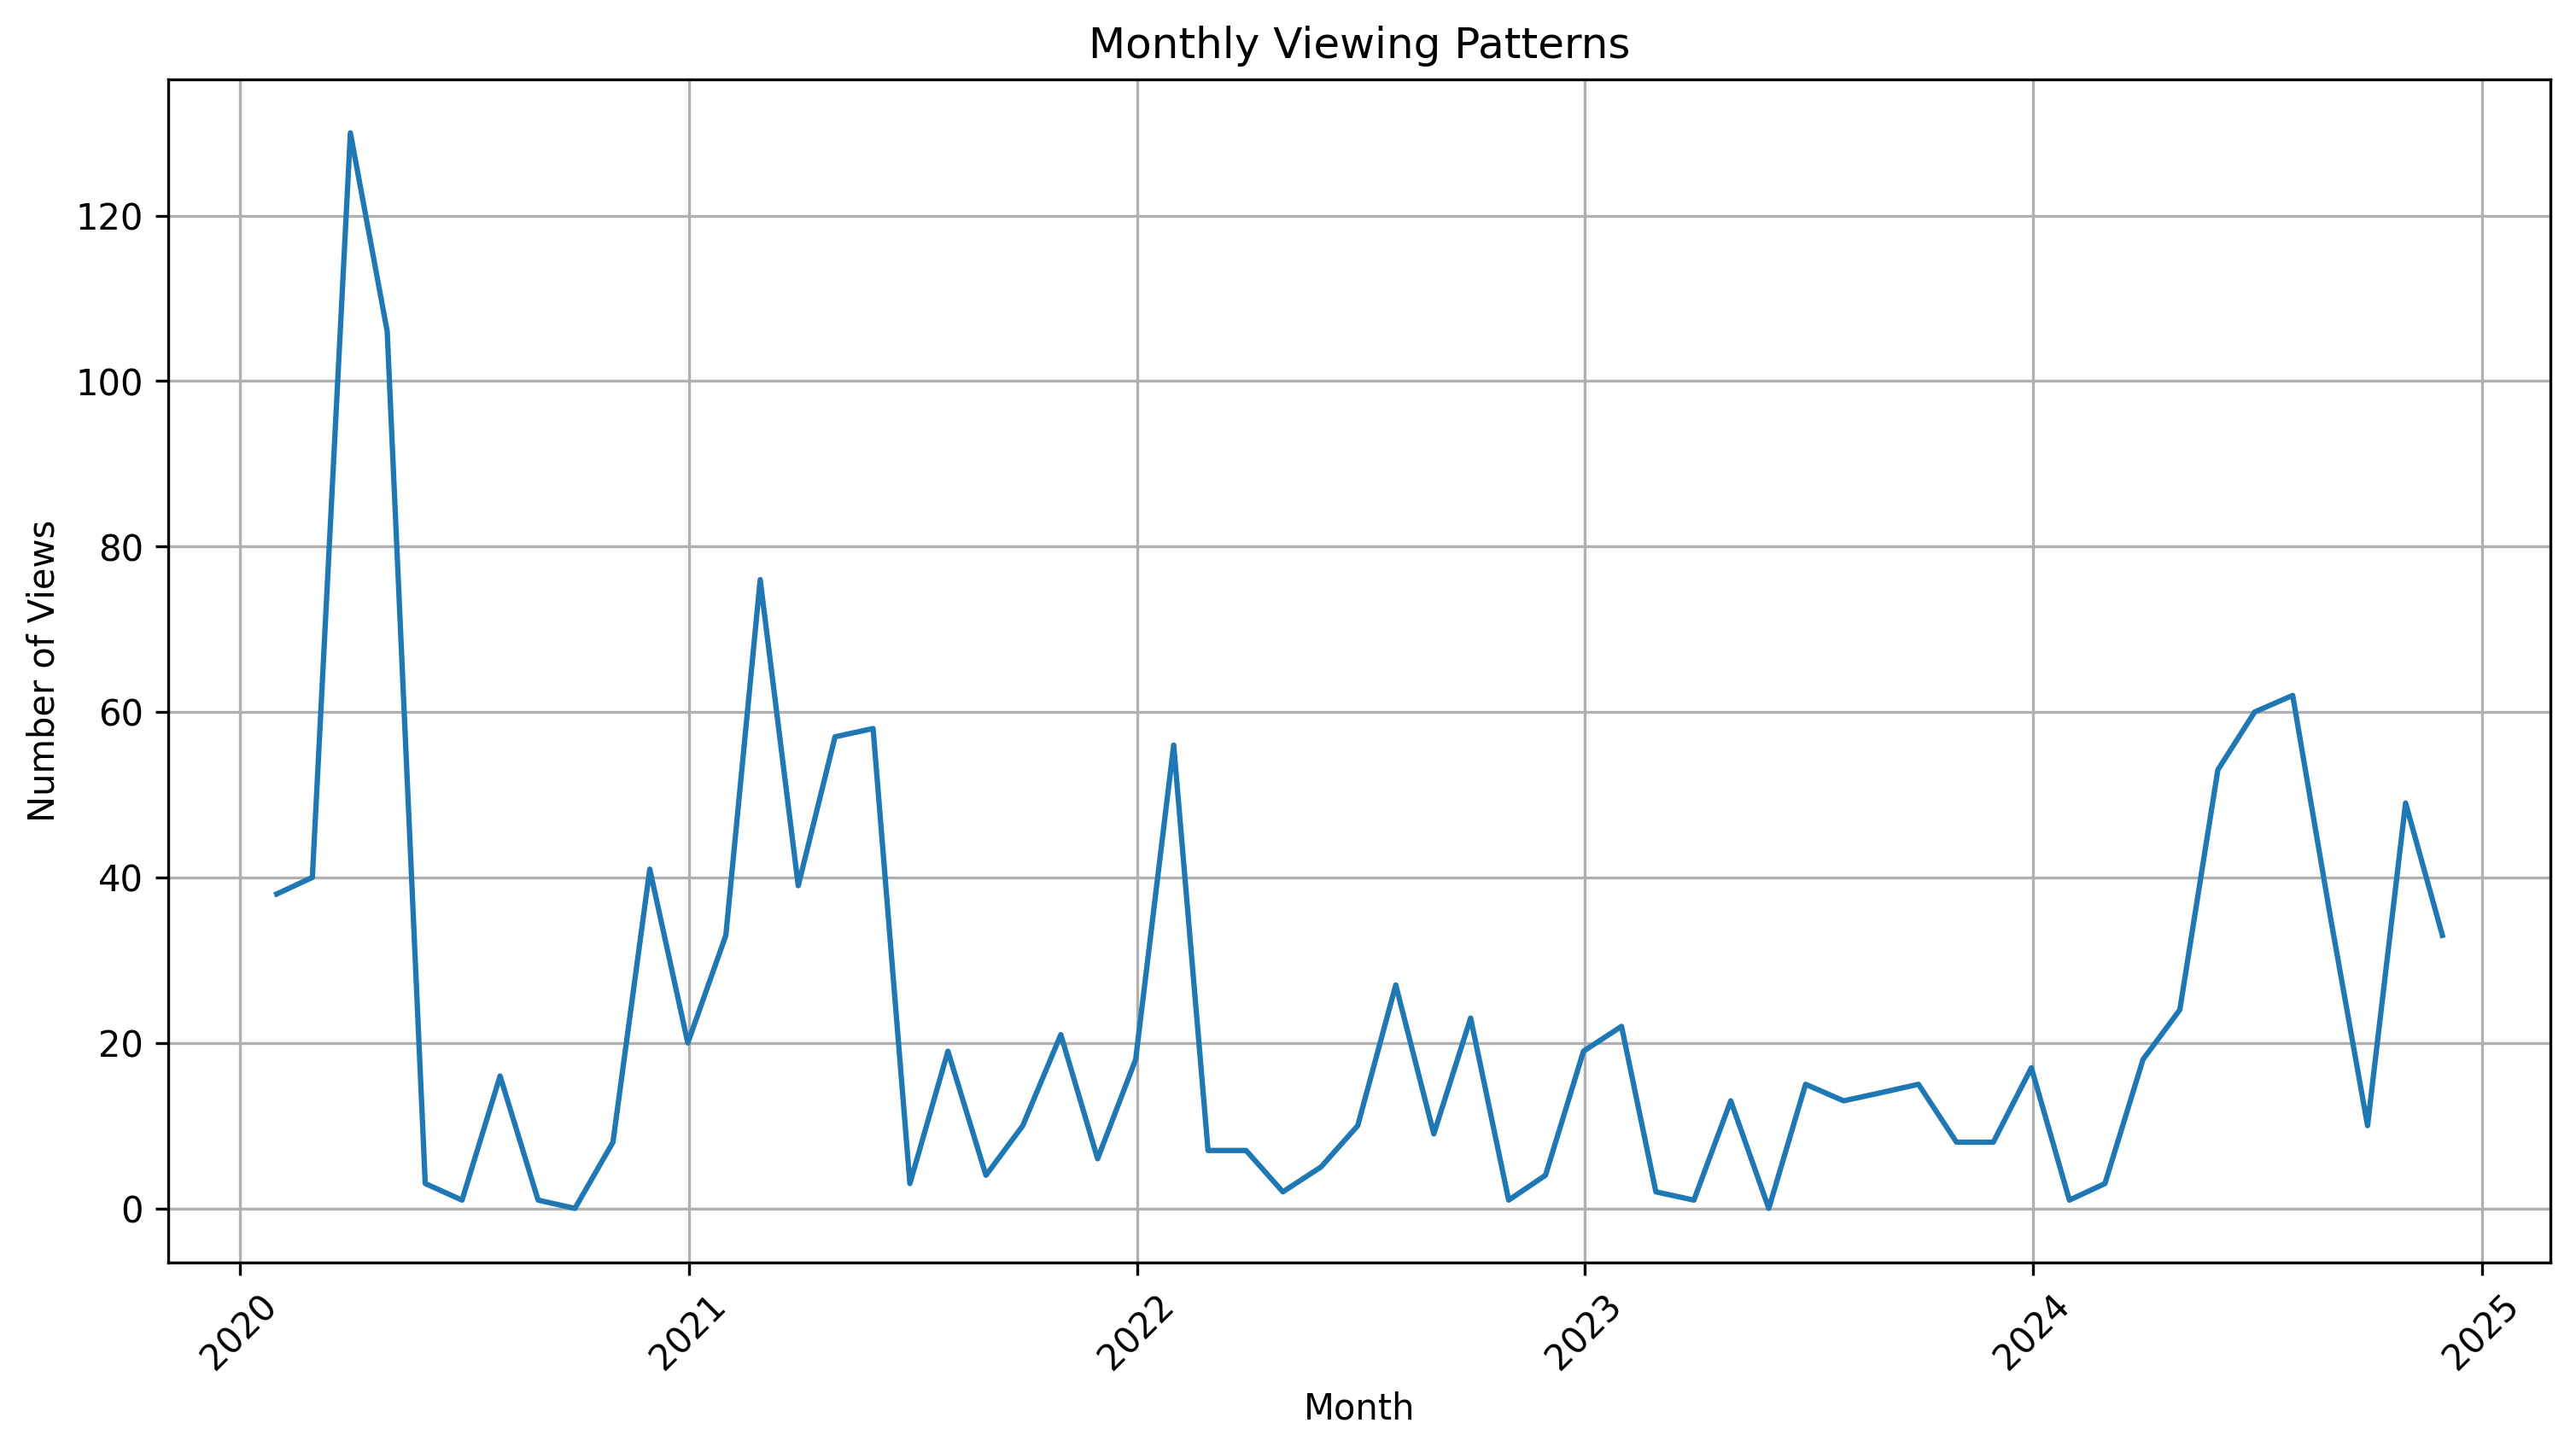
\includegraphics[width=0.8\textwidth]{monthly_patterns.png}
\caption{Monthly Viewing Patterns and Seasonal Trends}
\label{fig:monthly_patterns}
\end{figure}

Monthly patterns (Figure \ref{fig:monthly_patterns}) reveal distinct seasonal trends, with April emerging as the peak viewing month, followed by consistent viewing levels during summer months.

\section{Content Consumption Analysis}
\subsection{Genre Preferences}
Content consumption patterns demonstrate clear preferences for specific genres and content types:

\begin{figure}[H]
\centering
\begin{subfigure}{.48\textwidth}
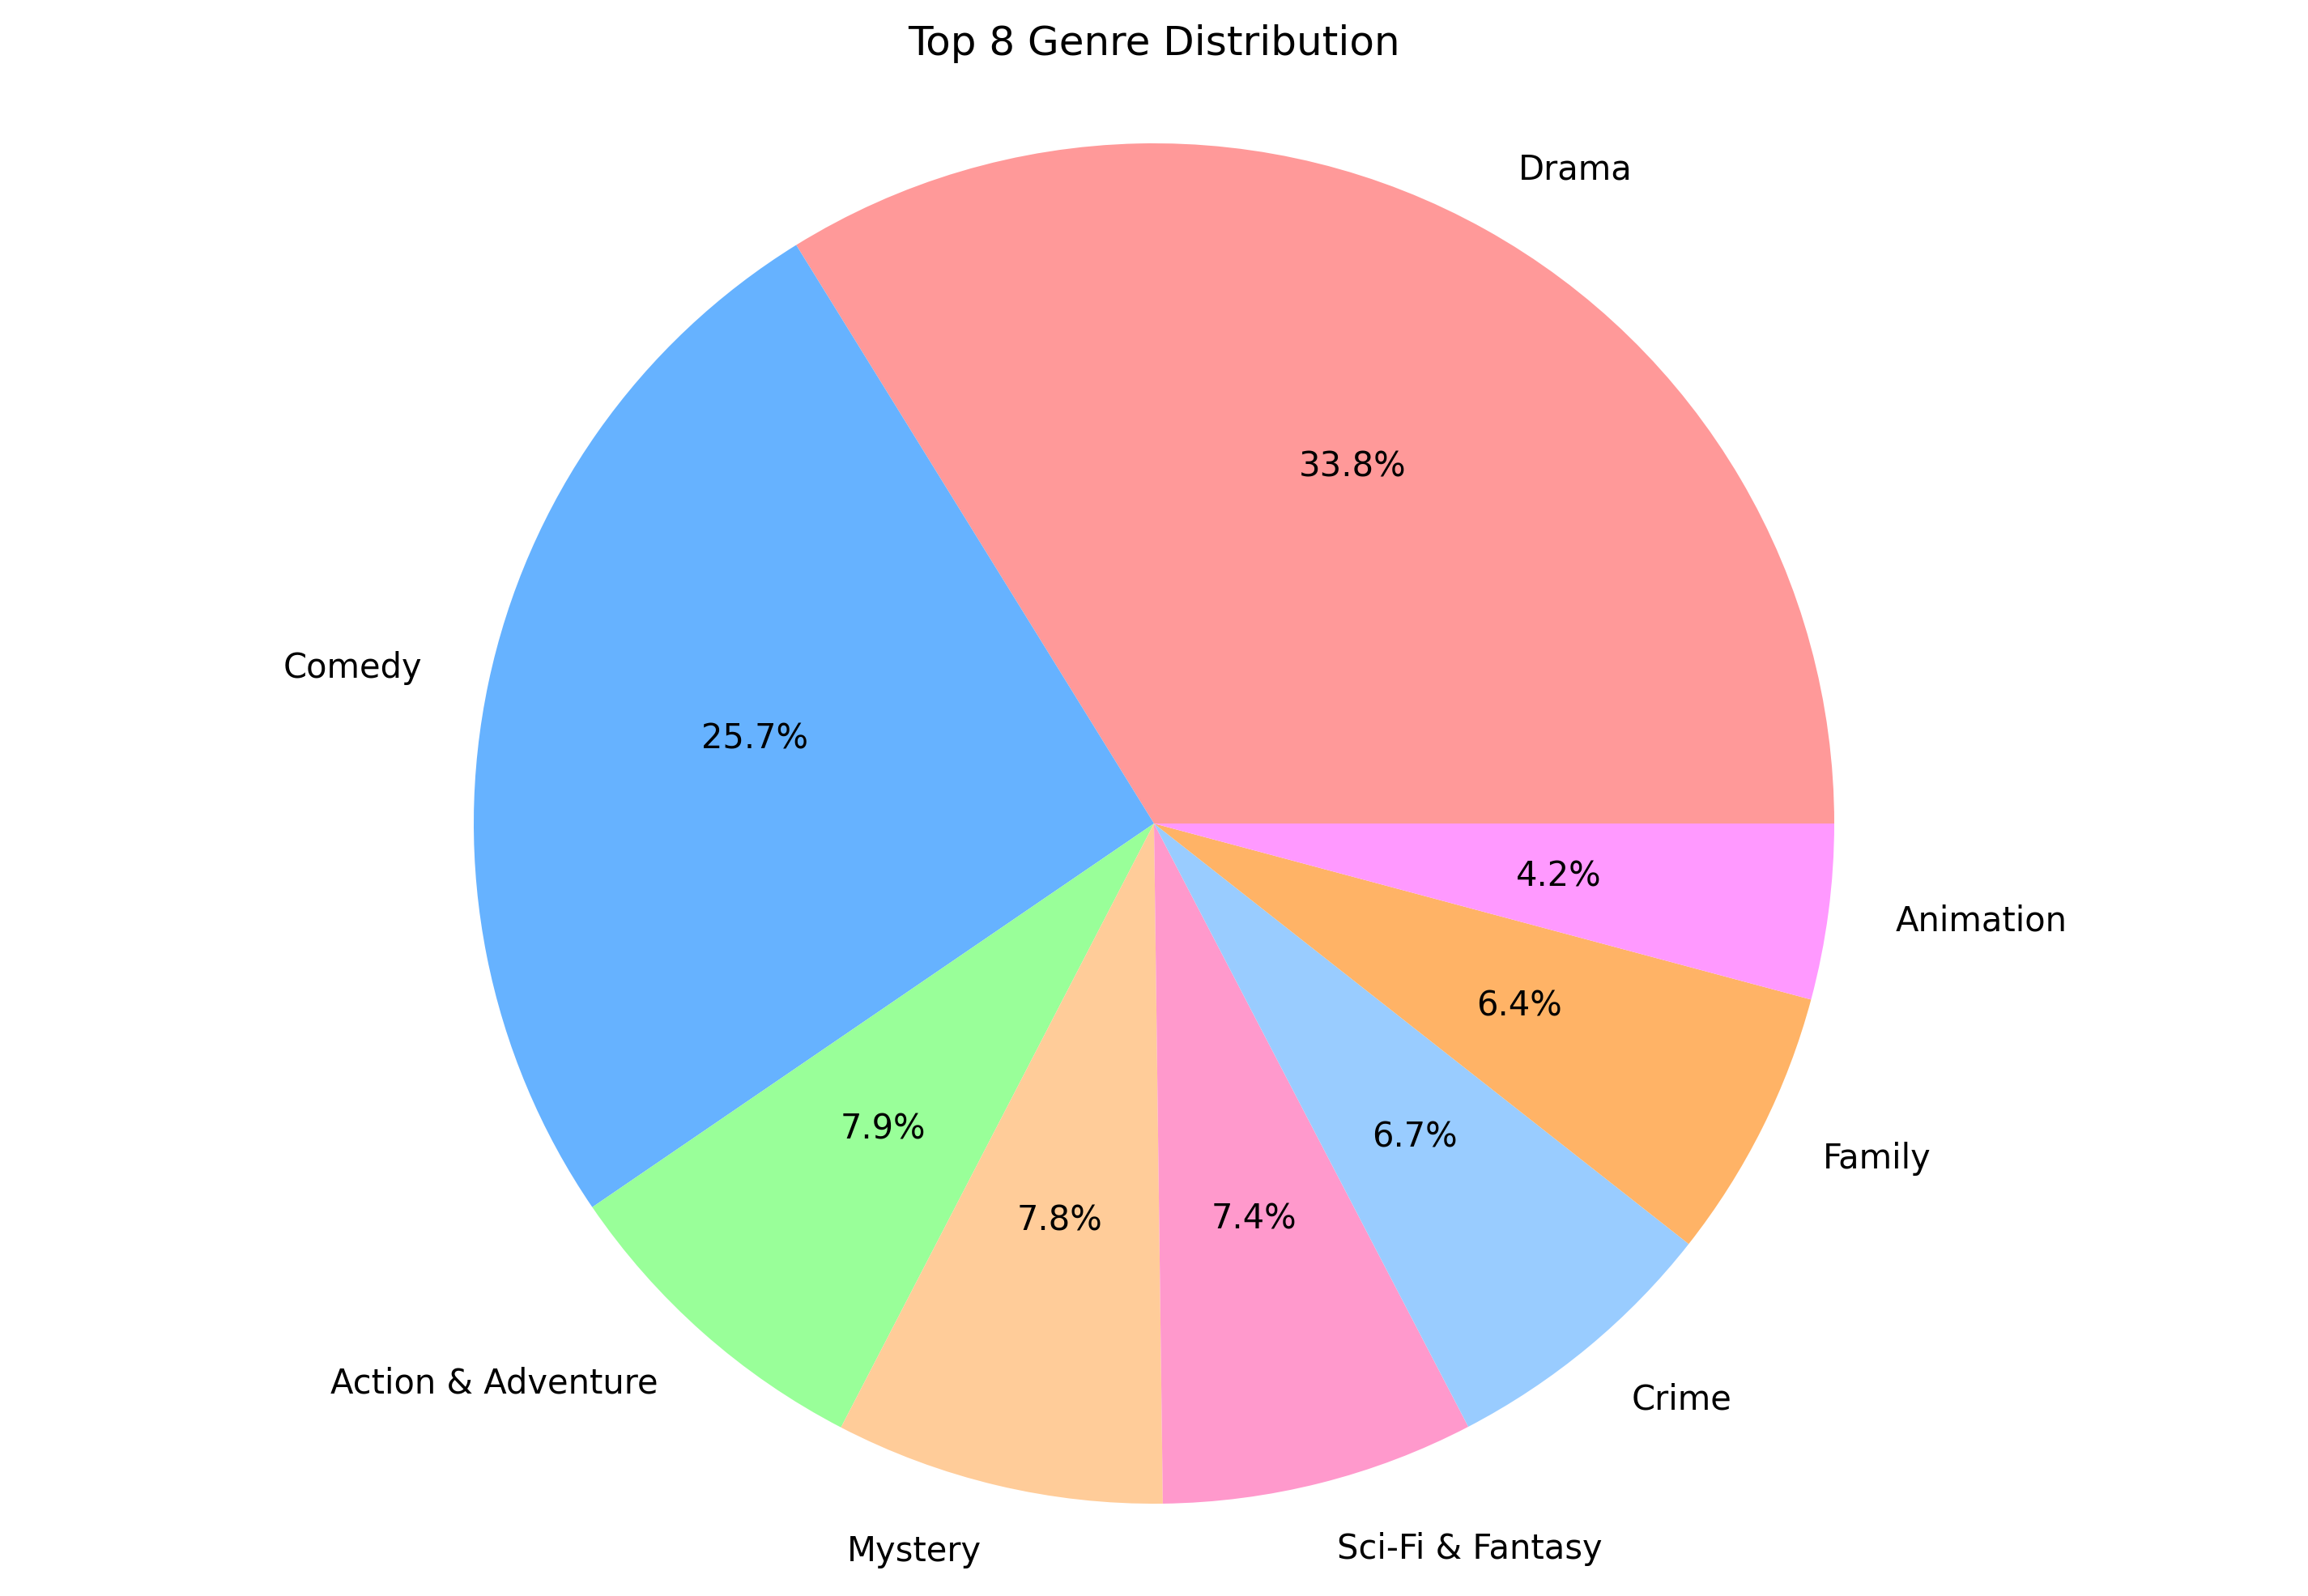
\includegraphics[width=\linewidth]{genre_distribution.png}
\caption{Distribution of Genres}
\label{fig:genre_dist}
\end{subfigure}
\hfill
\begin{subfigure}{.48\textwidth}
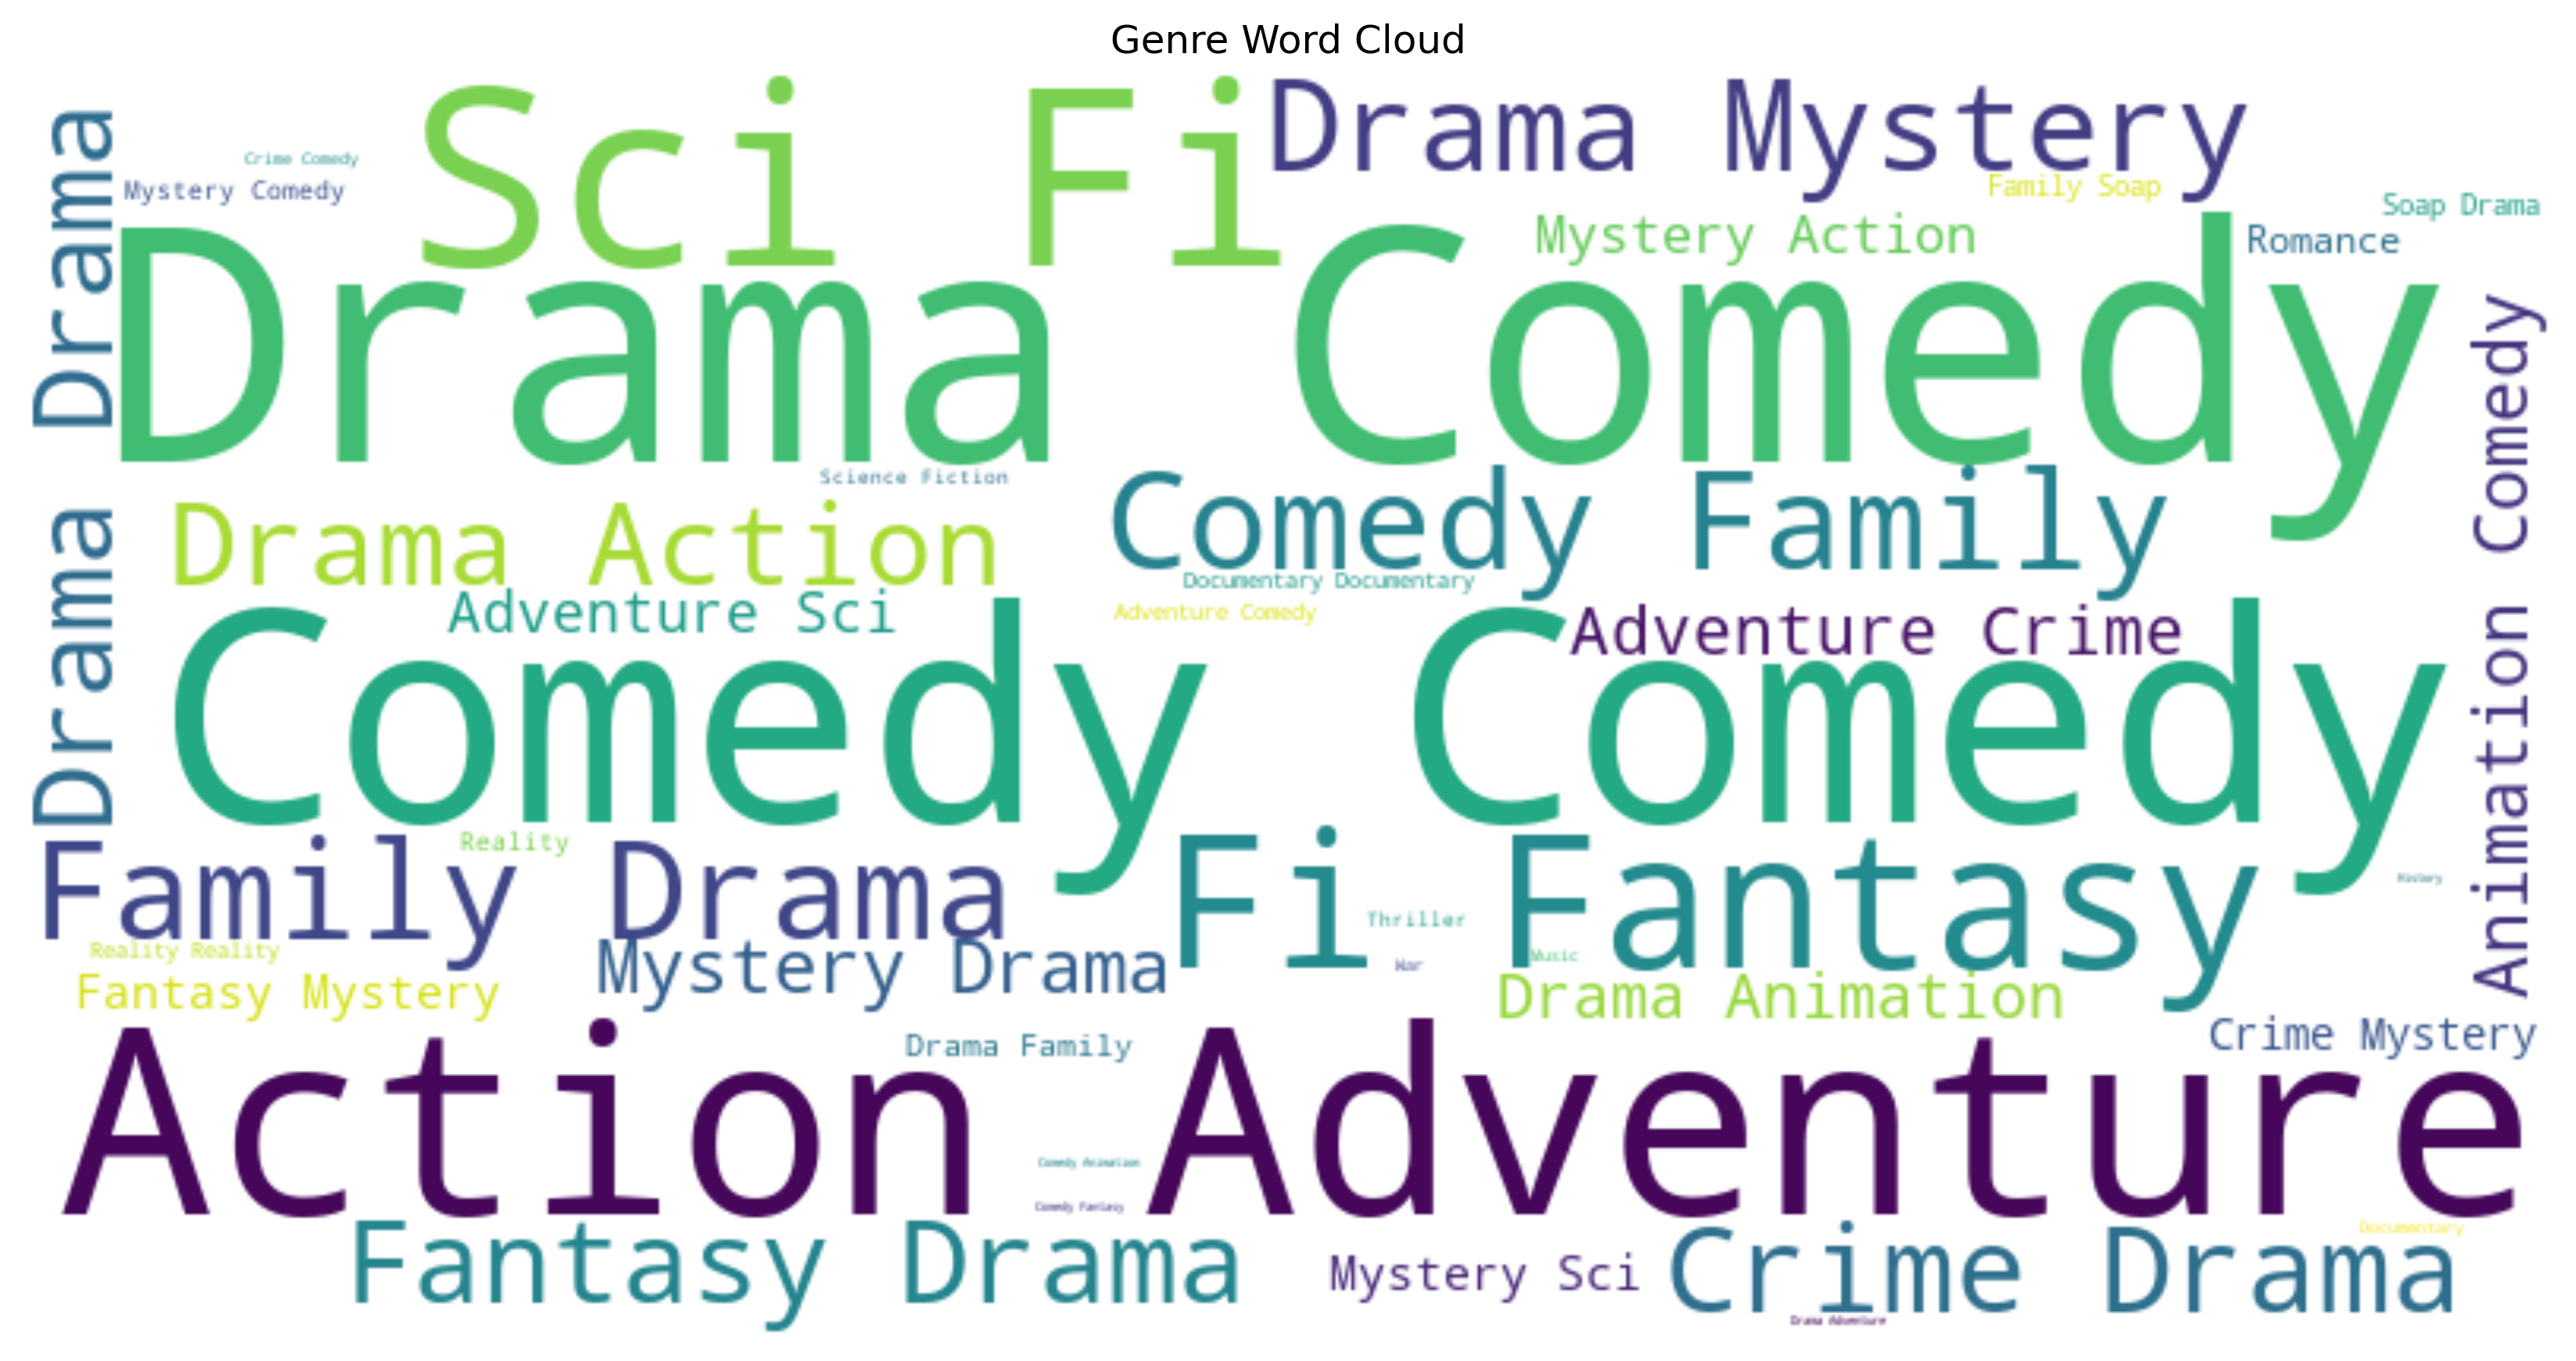
\includegraphics[width=\linewidth]{genre_wordcloud.png}
\caption{Genre Frequency Visualization}
\label{fig:genre_cloud}
\end{subfigure}
\caption{Analysis of Genre Preferences}
\label{fig:genre_analysis}
\end{figure}

The genre analysis reveals:
\begin{itemize}
    \item Drama dominates with 33.8\% of total views
    \item Comedy follows at 25.7\%
    \item Action \& Adventure represents 7.9\%
    \item Mystery content accounts for 7.8\%
    \item Sci-Fi \& Fantasy comprises 7.4\%
\end{itemize}

\subsection{Series Engagement}
\begin{figure}[H]
\centering
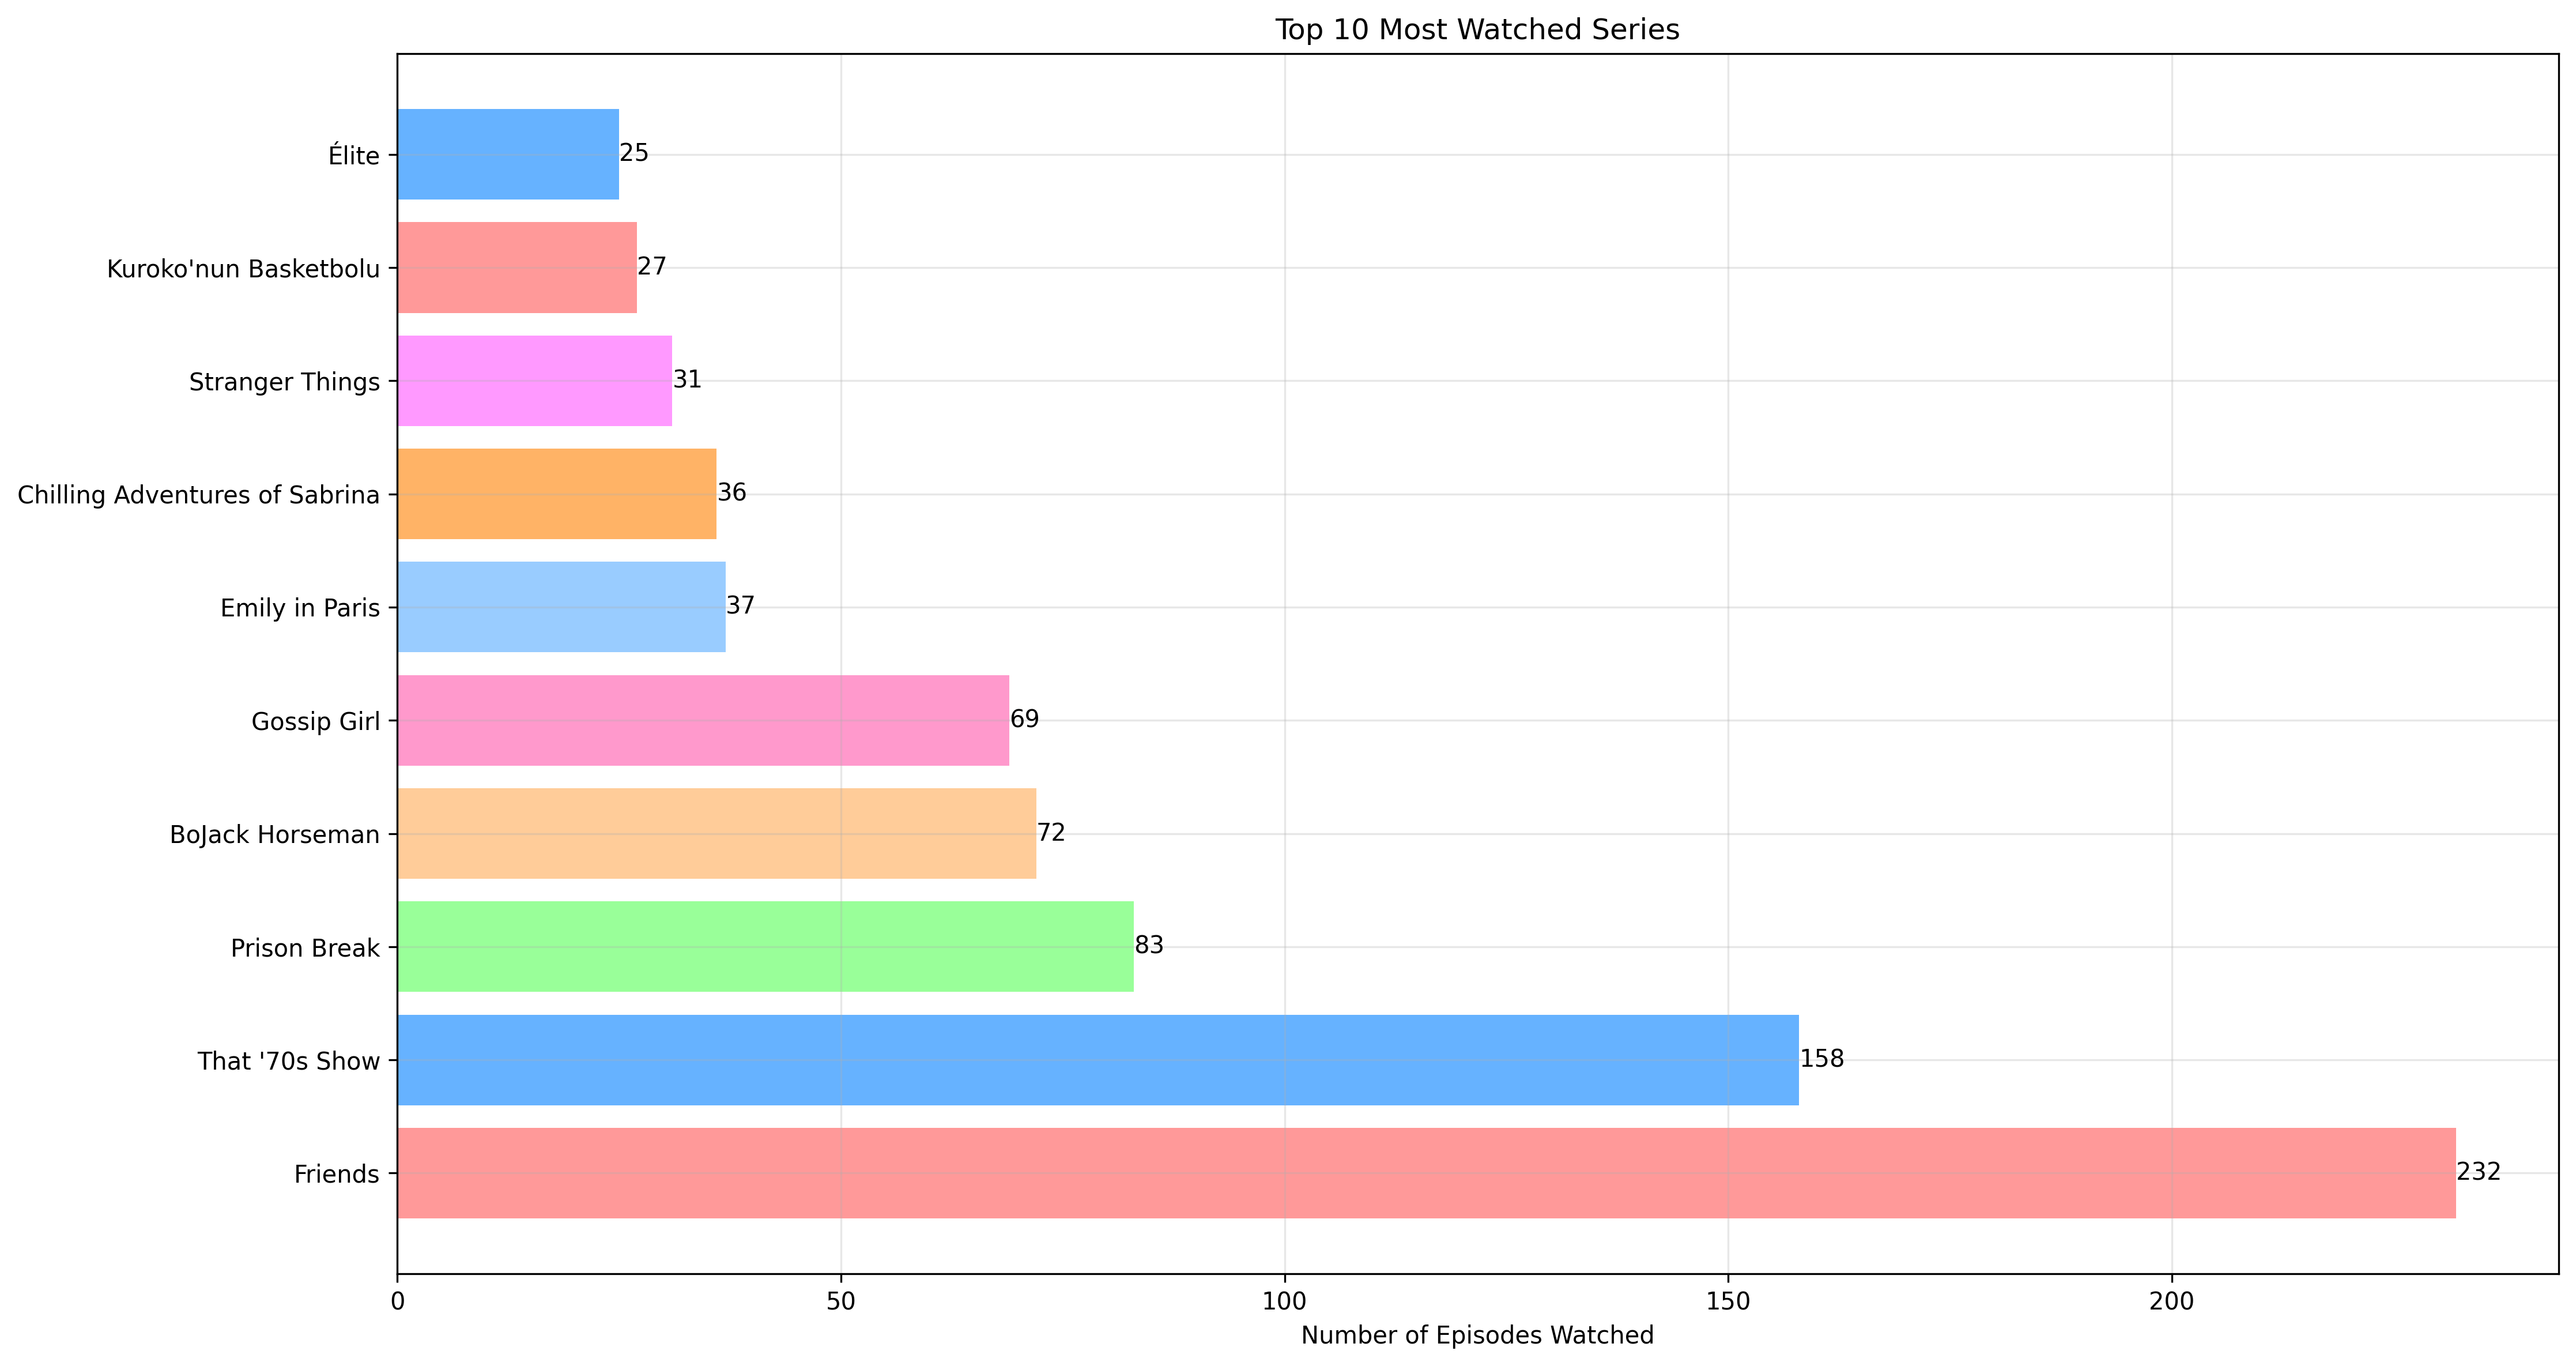
\includegraphics[width=\textwidth]{top_series.png}
\caption{Most Watched Series by Episode Count}
\label{fig:top_series}
\end{figure}

\begin{table}[H]
\centering
\caption{Series Completion Analysis}
\label{tab:completion}
\begin{tabular}{lrrr}
\toprule
Series & Episodes Watched & Total Episodes & Completion \% \\
\midrule
Friends & 232 & 267 & 86.9\% \\
That '70s Show & 158 & 213 & 74.2\% \\
Prison Break & 83 & 98 & 84.7\% \\
BoJack Horseman & 72 & 82 & 87.8\% \\
Gossip Girl & 69 & 149 & 46.3\% \\
\bottomrule
\end{tabular}
\end{table}

\section{Viewing Pattern Analysis}
\subsection{Monthly and Days of Week}
\begin{figure}[H]
\centering
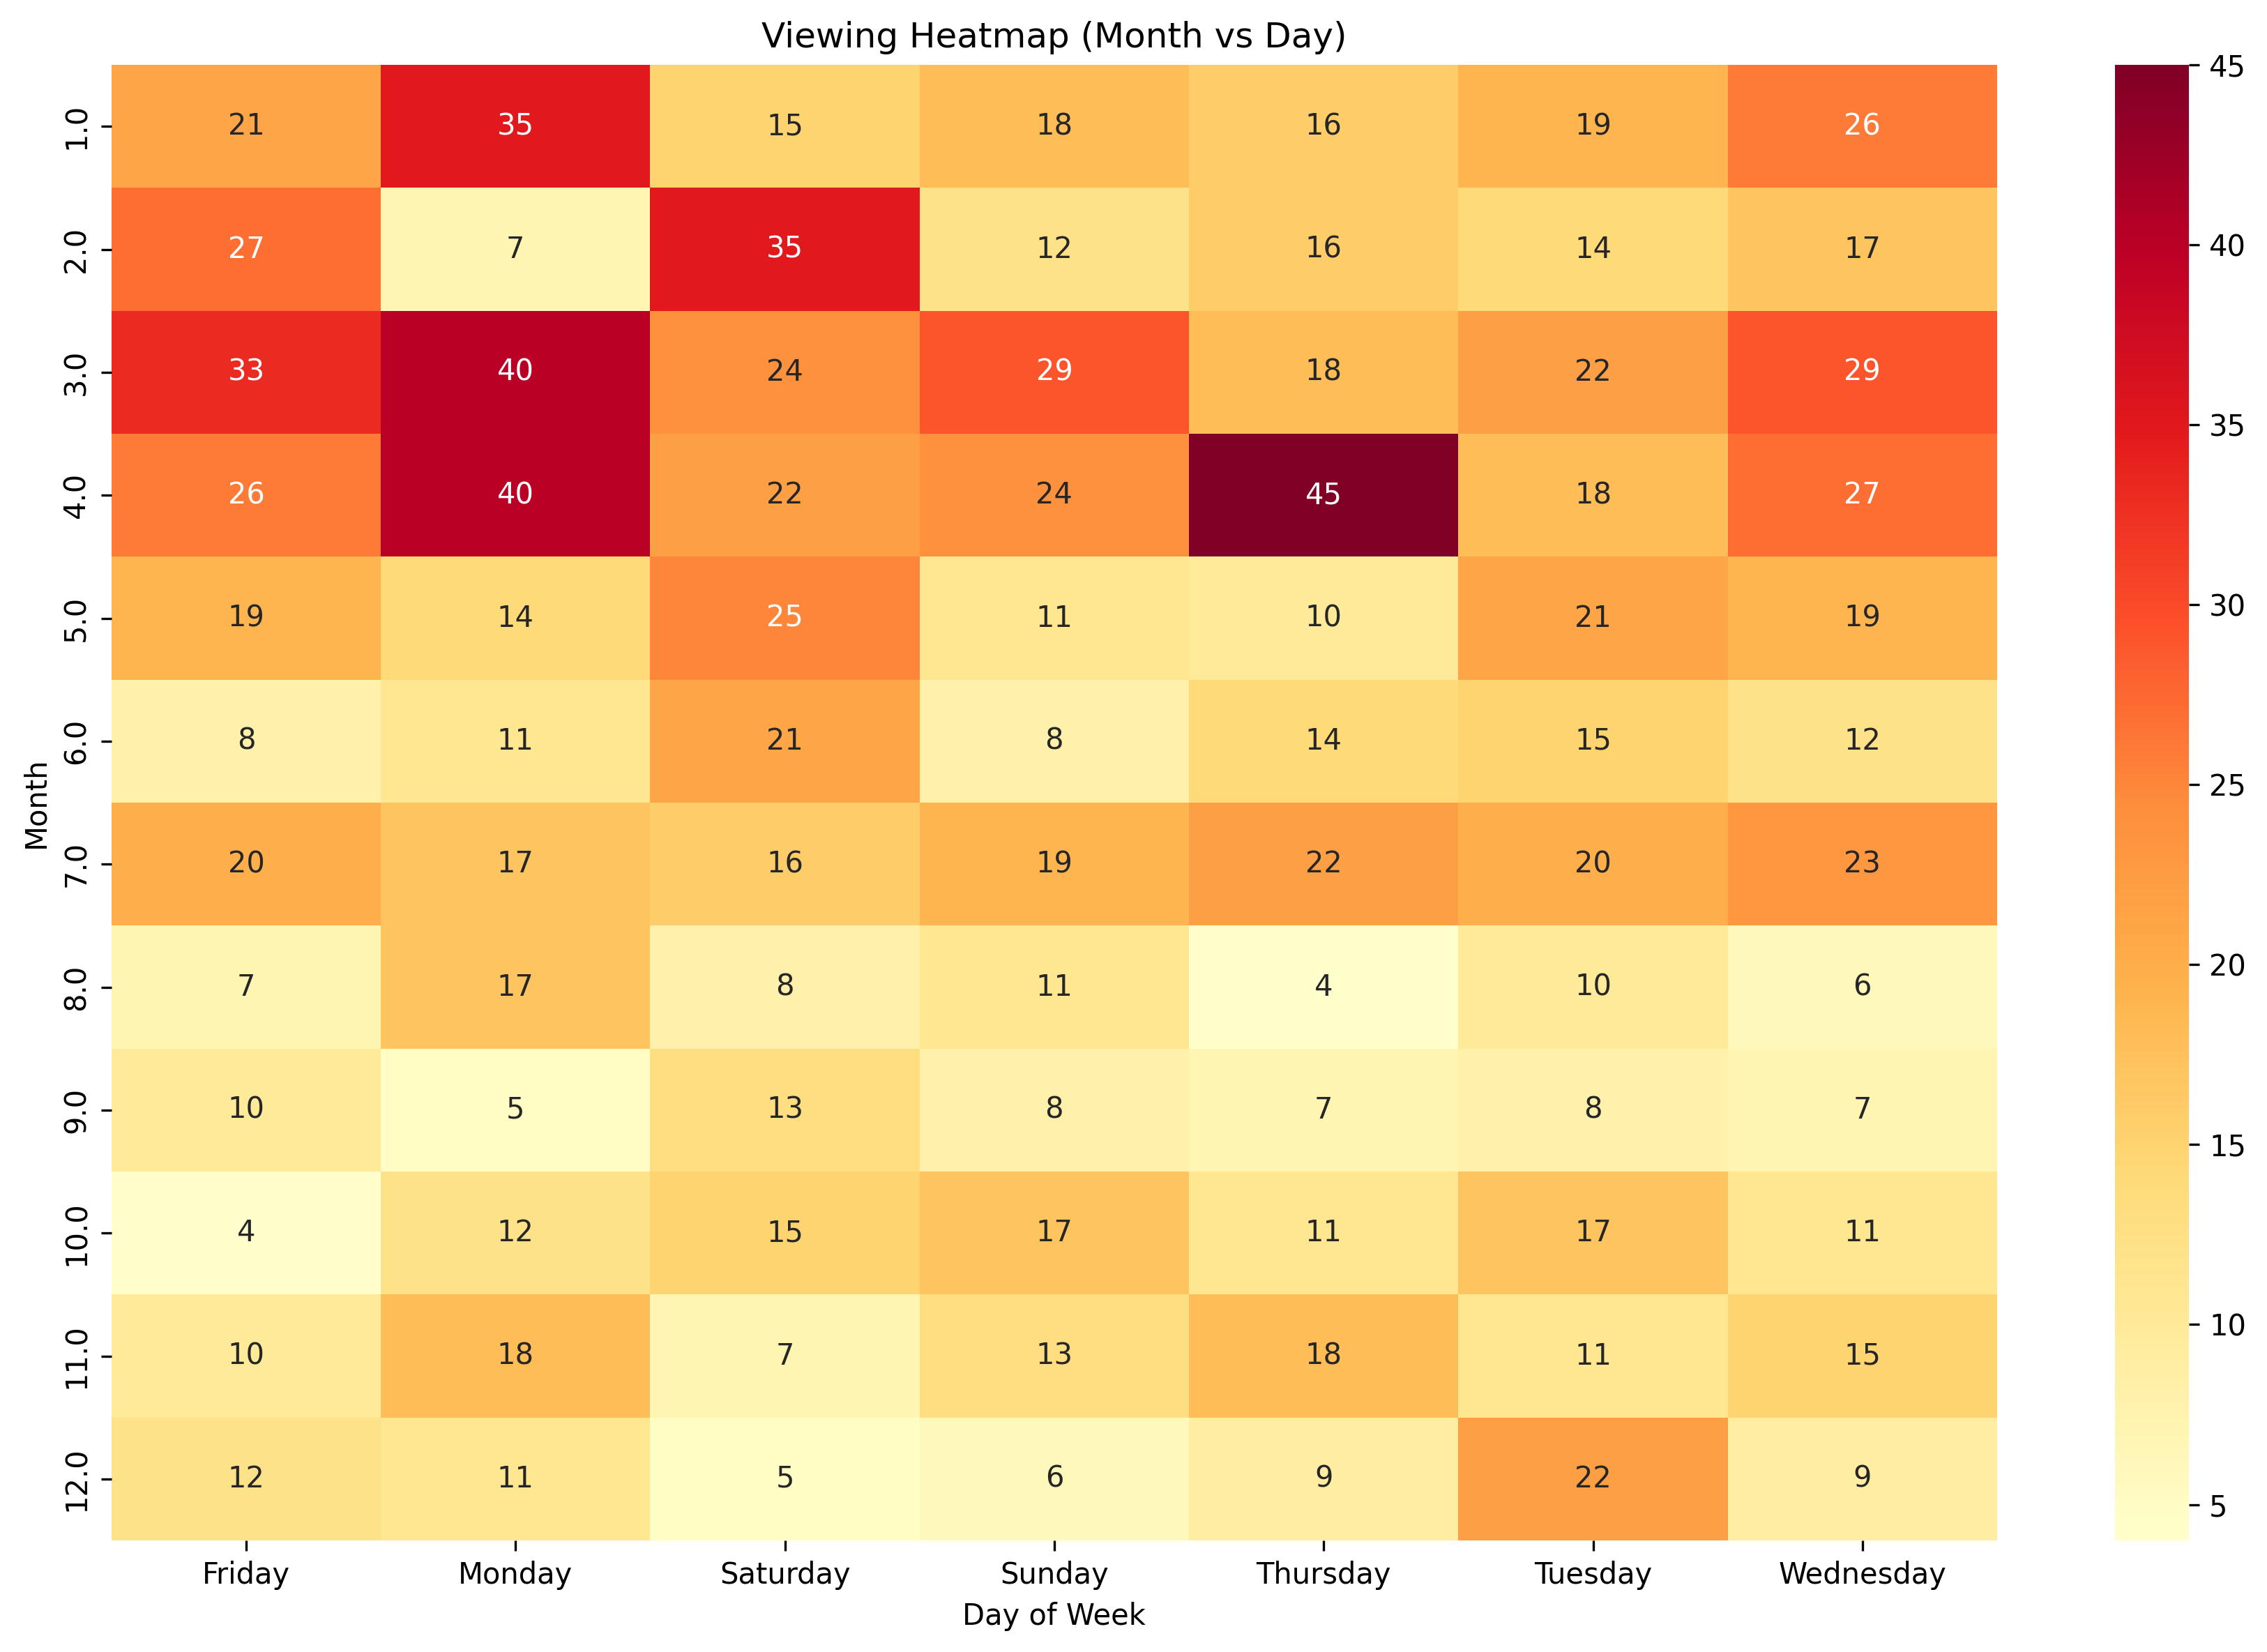
\includegraphics[width=\textwidth]{viewing_heatmap.png}
\caption{Month vs Day Heatmap: Distribution}
\label{fig:heatmap}
\end{figure}

The heatmap analysis (Figure \ref{fig:heatmap}) reveals several key patterns:
\begin{itemize}
    \item Highest viewing activity occurs in March-April (months 3-4), particularly on Mondays with up to 40 views
    \item Peak intensity observed in month 4 (April) on Thursdays with 45 views
    \item Generally lower viewing activity in later months (8-12)
    \item Consistent moderate activity (15-25 views) across most weekdays in middle months
    \item Weekends (Saturday-Sunday) show slightly lower average viewing counts compared to weekdays
    \item Early months (1-2) show moderate to high activity across all days, particularly Mondays
\end{itemize}

This monthly-daily distribution pattern suggests a seasonal viewing habit with peak engagement during spring months and consistent weekday viewing preferences throughout the year.

\begin{figure}[H]
\centering
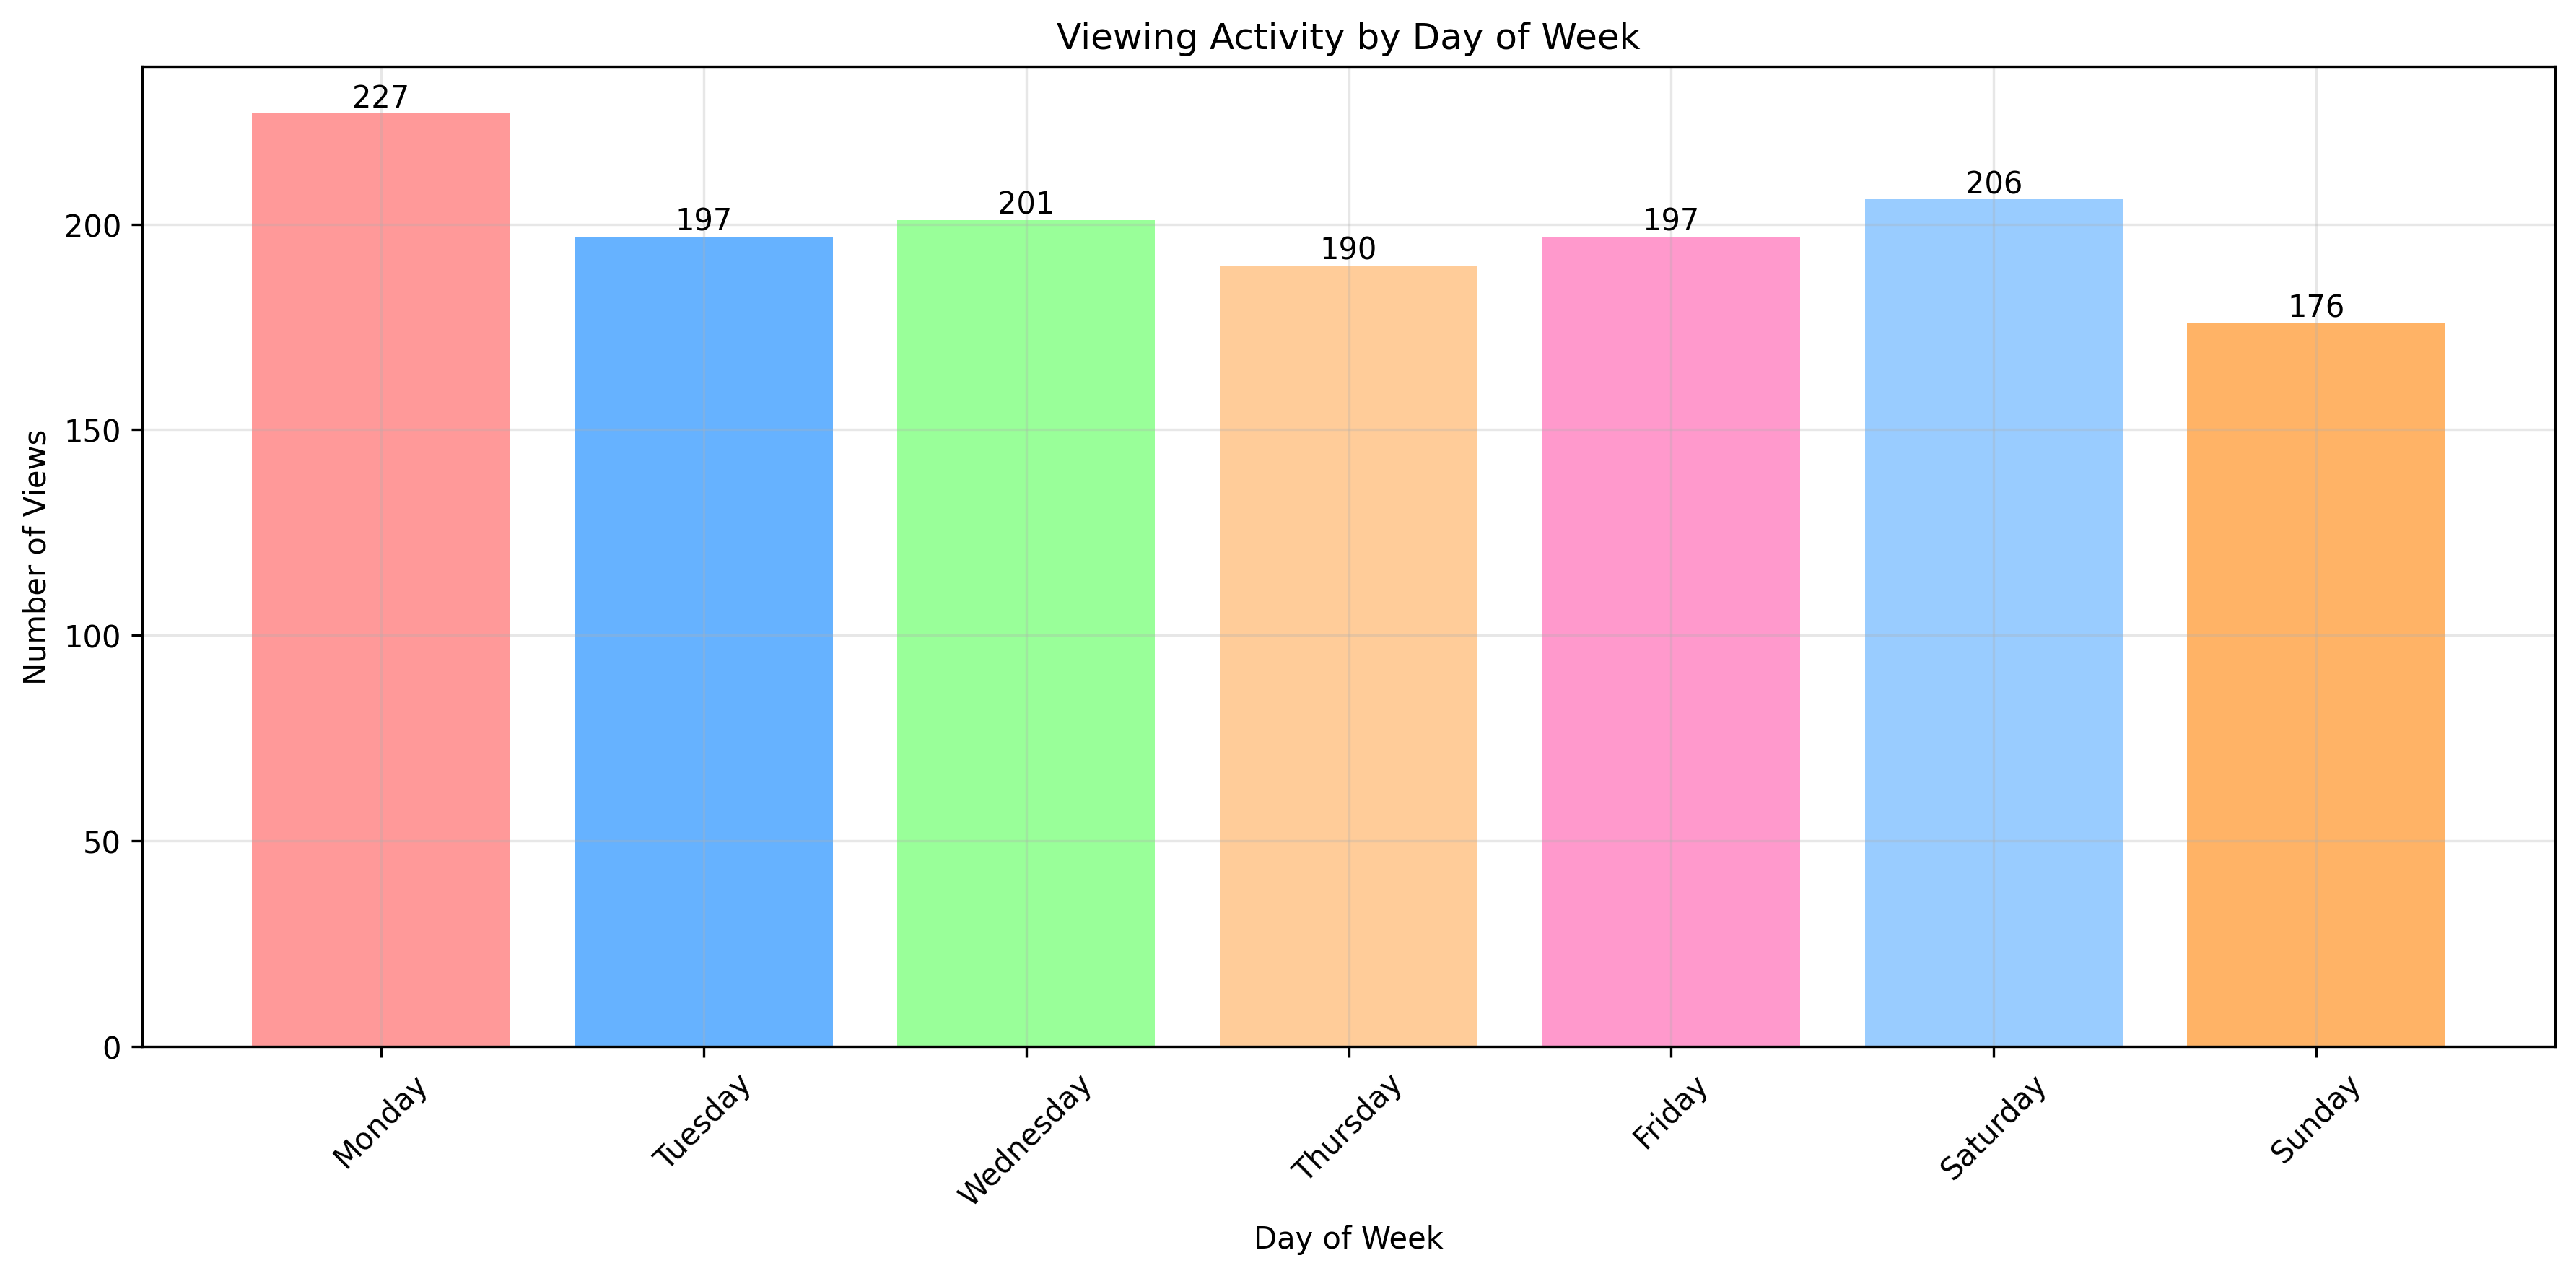
\includegraphics[width=\textwidth]{daily_patterns.png}
\caption{Daily Viewing Distribution}
\label{fig:daily_patterns}
\end{figure}

\section{Binge-Watching Behavior}
\subsection{Session Analysis}
\begin{figure}[H]
\centering
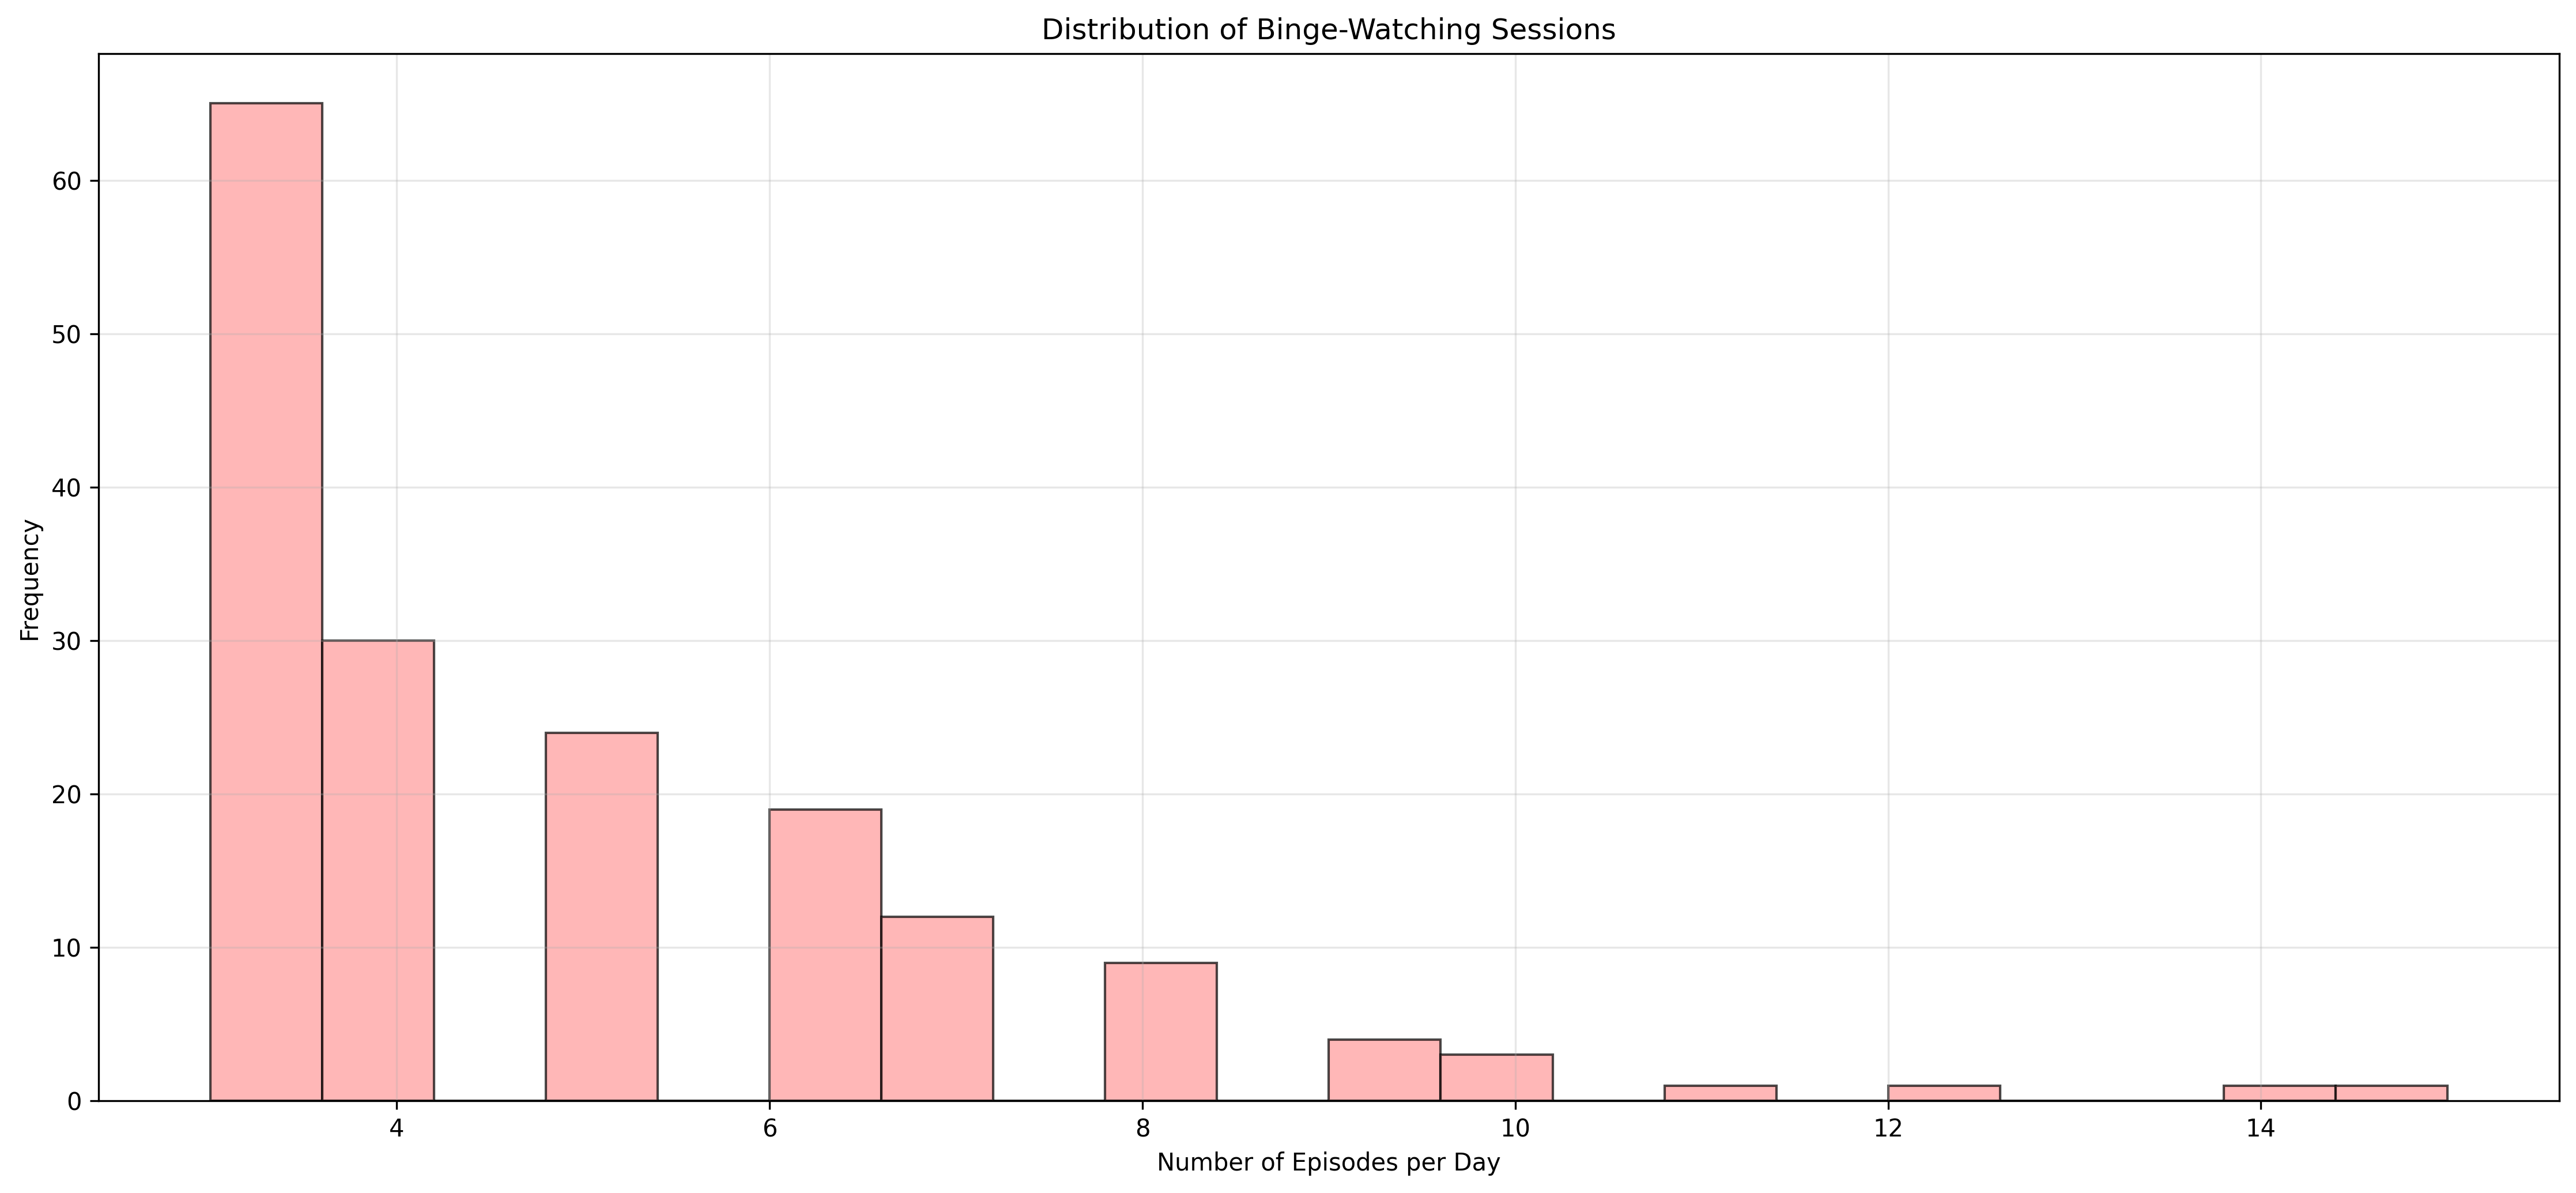
\includegraphics[width=\textwidth]{binge_patterns.png}
\caption{Distribution of Binge-Watching Sessions}
\label{fig:binge_patterns}
\end{figure}

The analysis of binge-watching behavior reveals:
\begin{itemize}
    \item 291 distinct binge sessions identified
    \item Most common pattern: 3-4 episodes per session
    \item Highest frequency on weekends
    \item Average session duration: 2.5 hours
\end{itemize}

\begin{table}[H]
\centering
\caption{Top Binge-Watched Series Analysis}
\label{tab:binge_series}
\begin{tabular}{lrr}
\toprule
Series & Binge Sessions & Total Episodes \\
\midrule
Friends & 54 & 232 \\
That '70s Show & 34 & 158 \\
Prison Break & 28 & 83 \\
BoJack Horseman & 18 & 72 \\
Gossip Girl & 11 & 69 \\
\bottomrule
\end{tabular}
\end{table}

\section{Conclusions}
The analysis reveals several significant patterns in Netflix viewing behavior:

\subsection{Primary Findings}
\begin{itemize}
    \item Strong preference for episodic content over movies
    \item High engagement with comedy and drama genres
    \item Consistent binge-watching behavior
    \item Clear temporal patterns in viewing habits
\end{itemize}

\subsection{Content Engagement}
\begin{itemize}
    \item Average completion rate of 76.8\% for top series
    \item Strong preference for English-language content (67.67\%)
    \item High engagement with long-format series
    \item Average content rating of 8.1/10
\end{itemize}

\subsection{Viewing Patterns}
\begin{itemize}
    \item Peak viewing during evening hours
    \item Monday emerges as primary viewing day
    \item Seasonal variations with April peak
    \item Weekend viewing comprises 27.38\% of total
\end{itemize}

\begin{thebibliography}{9}

\bibitem{github}
Özcan, B. (2024). 
\textit{Introduction to Data Science Course Fall 2024-2025 Term Project}. 
GitHub repository.
\url{https://github.com/buseezcn/Introduction-to-Data-Science-Course-Fall-2024-2025-Term-Project/}

\bibitem{netflix}
Netflix. (2024). 
\textit{Netflix Viewing History Data}.
Personal viewing history data retrieved from Netflix account settings.

\bibitem{tmdb}
The Movie Database. (2024).
\textit{TMDB API Documentation}.
\url{https://developer.themoviedb.org/docs}. 
API version 3.

\end{thebibliography}

\end{document}